\subsection{Необходимость}
Однопроцессорная версия алгоритма имеет весьма ограниченную применимость: основным ограничивающим фактором является объём оперативной памяти, доступной на локальном вычислительном узле. Границы применимости однопроцессорной версии можно получить при помощи следующих предположений:
\begin{itemize}
	\item используемые типы данных -- float (4 байта) и int (4 байта);
	\item в каждом узле сетки хранится 3 значения вектора скорости, 6 значений тензора, по 3 значения координат в локальной и подвижной системах, 4 значения параметров реологии среды;
	\item в процессе расчёта каждого временного шага требуется хранить копию расчётов предыдущего временного слоя, для записи результатов на жёсткий диск необходима третья копия;
	\item каждый узел хранит информацию о <<локальной>> топологии сетки для быстрого доступа к соседним тетраэдрам и треугольникам (в среднем по пять значений типа int для каждого типа элементов).
\end{itemize}

Суммарно имеем следующий расход памяти на хранения одного узла: 228 байт. В этих расчётах не учитываются расходы на хранения топологии всей сетки, ввиду сложности проведения оценки. Таким образом получаем, что при доступном объёме памяти в 1 Гб для одного вычислительного узла с максимальной скоростью можно проводить расчёты на сетках с числом узлов \todo{Эта цифра немного не сходится с расчётами выше}1-2 миллиона. Под максимальной скоростью здесь понимается следующее: при расчёте на сетках указанного выше размера все необходимые данные могут быть полностью помещены в оперативной памяти, скорость доступ к которой на порядки выше скорости чтения с жёсткого диска.

Характерный размер сетки для решаемый задачи — \todo{Посчитать объём точнее} 792000 узлов (11 слоёв, каждый из которых имеет размер 120x120x5). Стоит отдельно отметить, что размеры этой задачи лежат на самой нижней границе характерных размеров задач, решение которых представляет практический интерес. Поставленную задачу уже весьма проблематично решить на одном вычислительном узле ввиду ограниченного размера доступной для вычислений оперативной памяти.

Другой причиной необходимости создания параллельной версии алгоритма является характер роста вычислительной сложности при увеличении числа узлов сетки ($O(n^3)$). Отсюда следует, что при уменьшении характерных размеров задачи вдвое сложность вычислений возрастает в 8 раз. Очевидно, что задачи такого класса необходимо решать при помощи параллельных версий алгоритмов, чтобы обеспечить хотя бы небольшую масштабируемость.

Таким образом создание параллельной версии алгоритма становится необходимым условием численного моделирования задач подобного рода.

\subsection{Способ построения параллельной версии}
Для реализации параллельных вычислений исходная геометрия разбивается на зоны, которые распределяются между вычислительными узлами. Один узел может производить одновременный расчёт нескольких зон. Для обеспечения согласованности расчёта вычислительные узлы обмениваются необходимой информацией о значениях и топологии сеток на границах зон. Для получения максимальной эффективности при параллельном расчёте следует учитывать следующие условия:
\begin{itemize}
	\item для увеличения времени полезного использования кластера необходимо, чтобы время расчёта очередного временного слоя на каждом вычислительном узле было примерно одинаково, так как в противном случае наиболее <<быстрые>> узлы проводят некоторые время в ожидании, при этом не проводя никаких расчётов;
	\item для увеличения скорости синхронизации и расчёта контактных границ крайне желательно, чтобы зоны имели простую геометрию;
	\item граничные части сеток различных зон должны быть построены согласованно (в идеале должны совпадать топологически) для уменьшения потерь точности, связанных с интерполяцией;
	\item расчёт каждого временного слоя должен быть максимально <<параллельным>> в том смысле, что синхронизации происходят редко и согласованно, а данные передаются большими объёмами.
\end{itemize}
\subsubsection{Тестирования производительности MPI}
\todo{Почему именно MPI?}Для выбора правильных API для построения параллельной версии был проведён ряд тестов производительности обмена сообщениями при помощи MPI. Одним из наиболее важных вопросов, ответ на которых хотелось получить был следующий: каков оптимальный объём сообщения для пересылки? Иными словами, нужно было выяснить, при каких размерах посылаемого сообщения время, затрачиваемое на пересылку одного байта, минимально.
Ниже приведены графики (см. рис. \ref{mpi1host} и рис. \ref{mpi2hosts} зависимости затрат на пересылку одно байта в зависимости от размера сообщения.
\begin{figure}[htp]
\centering
\includegraphics[width=0.6\textwidth]{eps/mpi-1host.eps}
\caption{Затраты на пересылки при использовании одного вычислительного
 узла}
\label{pic:mpi1host}
\end{figure}
\begin{figure}[htp]
\centering
\includegraphics[width=0.6\textwidth]{eps/mpi-2hosts.eps}
\caption{Затраты на пересылки при использовании двух вычислительных узлов}
\label{pic:mpi2hosts}
\end{figure}
Как видно из графиков, для пересылки данных посредством MPI выгодно использовать большие объёмы сообщений. В первую очередь это связано с ростом доли накладных расходов на пересылку сообщения при уменьшении его размера. Другими факторами, снижающими скорость передачи, могут служить буферизация исходящих сообщения, а также блокировки вызывающего процесса при синхронной передаче данных. По результатам проведённых тестов были сделаны следующие выводы;
\begin{itemize}
	\item данные нужно передавать большими объёмами, так как скорость в таких случаях выше;
	\item следует использовать асинхронную передачу данных, возможно, с инициацией приёма до момента посылки данных;
	\item для ускорения процесса синхронизации крайне желательно использовать <<родные>> функции коллективного обмена данными вместо самостоятельной реализации подобного функционала;
	\item следует в полной мере использовать возможности MPI по созданию пользовательских типов данных для уменьшения объёмов памяти, требуемых для хранения временных структур данных, а также для уменьшения временн\'{ы}х затрат на копирование данных внутри вычислительного узла.
\end{itemize}

\subsubsection{Синхронизация шага по времени}
Перед расчётом очередного временного слоя необходимо синхронизировать шаг по времени между всеми вычислительными узлами. В текущей реализации метода с целью увеличения скорости расчёта вводится ограничение на максимально возможный шаг по времени:
\begin{equation}
\label{max_time_step}
\tau_{max}=\frac{h_{min}}{\lambda_{max}},
\end{equation}
где $h_{min}$ -- минимальная высота тетраэдра в сетке, а $\lambda_{max}$ -- максимальное значение коэффициента Ляме в локальной сетке. Так как для расчётов используются неструктурированные тетраэдральные сетки, максимально допустимый шаг по времени может различаться для разных зон. Поэтому в начале расчёта каждого временного слоя вычислительные узлы выбирают максимально допустимый шаг по времени для локальных сеток, после чего из выбирают минимальный из всех полученных. Дальнейший расчёт на всех вычислительных узлах ведётся с одним и тем же шагом по времени. Для выполнения этой операции крайне удобным оказалось использовать встроенную в MPI функцию коллективного обмена:\lstinputlisting[label=lst:time_step_sync,caption=Синхронизация шага по времени]{source/time_step_sync.cpp}
\subsubsection{Синхронизация узлов}
Как было сказано ранее, при параллельных вычисления исходная сетка делится между вычислительными узлами. При этом нередки ситуации, когда одно физическое тело <<разрезано>> на несколько зон. В этом случае получаем следующее: часть узлов, необходимых для расчёта сетки А, принадлежат сетке Б (см. рис. \ref{pic:remote_nodes}). Именно эти узлы (на этапе загрузки они помечаются как REMOTE) необходимо синхронизировать.
\begin{figure}[htp]
\centering
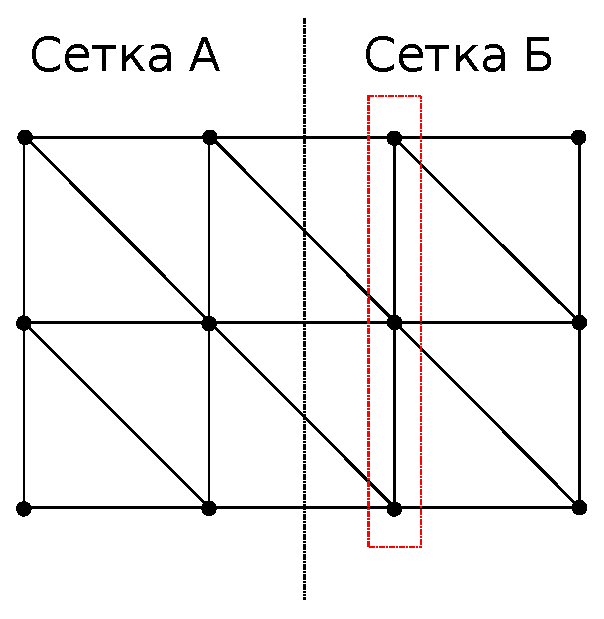
\includegraphics[width=0.4\textwidth]{eps/remote_nodes.eps}
\caption{REMOTE узлы на сетках}
\label{pic:remote_nodes}
\end{figure}
В текущей реализации не используется динамическое перестроение сеток, поэтому на протяжении всего расчёта набор REMOTE узлов не меняется. Это позволяет на этапе загрузки провести первичную обработку сеток, получить список REMOTE узлов для каждой пары сеток и создать пользовательские типы MPI для дальнейших пересылок между вычислительными узлами. Характерный код создания пользовательских типов MPI:
\lstinputlisting[label=lst:custom_types,caption=Создание пользовательских типов MPI]{source/custom_types.cpp}
После этого пересылка всех узлов выполняется так:
\lstinputlisting[label=lst:nodes_sync,caption=Синхронизация REMOTE узлов]{source/nodes_sync.cpp}
\subsubsection{Детектор столкновений}
Для решения поставленной задачи требуется реализовать параллельный алгоритм явного выделения контактных границ. Стандартный подход (именно он использован в этой работе) к реализации состоит из двух этапов:
\begin{itemize}
	\item грубое (\todo{Добавить подпись?}см. рис. \ref{pic:collision_detection}) определение областей потенциально возможного контакта при помощи AABB (Axis-aligned bounding box);
	\item уточнение контактирующих узлов внутри найденных областей.
\end{itemize}
\begin{figure}[htp]
\centering
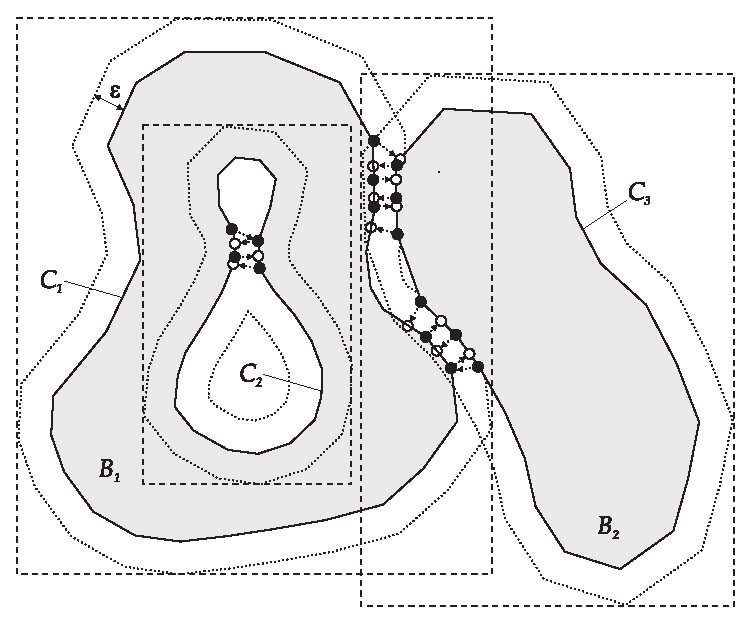
\includegraphics[width=0.6\textwidth]{eps/collision_detection.eps}
\caption{Использование AABB для грубого определения областей контакта}
\label{pic:collision_detection}
\end{figure}
Параллельная версия этого алгоритма устроена точно таким же образом. На первом шаге расчёта контактных границ все вычислительные узлы синхронизируют AABB локальных зон, для чего используется вызов стандартной функции MPI:
\lstinputlisting[label=lst:outlines_sync,caption=Синхронизация AABB]{source/outlines_sync.cpp}
После этого каждый вычислительный узел определяет пары <<потенциально>> находящихся в контакте зон -- одной локальной и одной удалённой. Затем для каждой найденной пары проводится уточнение зоны контакта: проверяются <<на контакт>> все пары локальных узлов и удалённых треугольников. Для этого проводится синхронизация треугольников, попавших в зону контакта. Идея здесь схожа с той, что используется при синхронизации удалённых узлов, но имеет некоторые отличия:
\begin{itemize}
	\item т.к. номера треугольников, попавших в зону контакта, заранее не известны, необходимо на первом шаге получить их;
	\item затем, чтобы использовать только одну пересылку на зону контакта, необходимо создать пользовательский тип MPI;
	\item последний шаг -- отправка найденных треугольников получателю.
\end{itemize}
После того, как все треугольники в зоне контакта получены с удалённого вычислительного узла, полным перебором определяются пары <<контактирующих>> узлов и треугольников. Под контактом точки и треугольника здесь понимается следующее: считаем, что треугольник и точка контактируют, если зона влияния (сфера заранее выбранного радиуса) точки пересекает треугольник (см. рис. \ref{pic:contact_detection}).
\begin{figure}[htp]
\centering
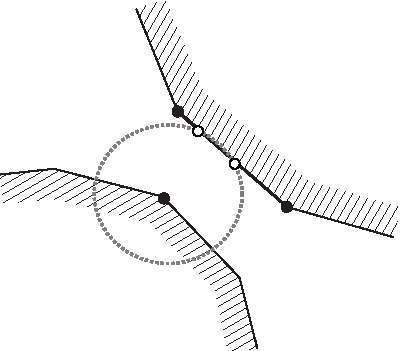
\includegraphics[width=0.6\textwidth]{pdf/contact_detection.pdf}
\caption{Определение контакта}
\label{pic:contact_detection}
\end{figure}
Если треугольник и точка находятся в контакте, то следующим шагом нужно построить парный виртуальный узел -- этот узел лежит внутри контактирующего треугольника так, чтобы прямая проходящая через реальный и виртуальный узлы, являлась нормалью к треугольнику (см. рис. \ref{pic:contact_processing}).
\begin{figure}[htp]
\centering
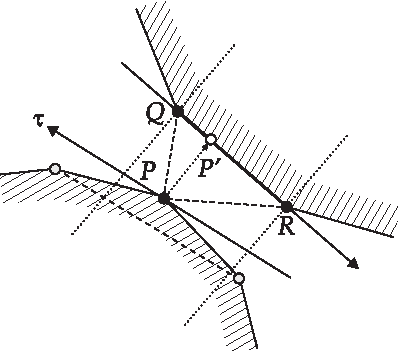
\includegraphics[width=0.6\textwidth]{pdf/contact_processing.pdf}
\caption{Построение виртуальных узлов при обработке контактирующих границ}
\label{pic:contact_processing}
\end{figure}
После того, как виртуальный узел построен, необходимо получить значения всех величин в нём. Для этого в данной работе использовалась линейная интерполяция при помощи барицентрических координат. Задача заключается в следующем (см. рис. \ref{pic:triangle_interpolation}): есть треугольник и точка, лежащая в его плоскости, в трёхмерном пространстве, нужно, используя известные значения в вершинах треугольника, определить значение в в точке.
\begin{figure}[htp]
\centering
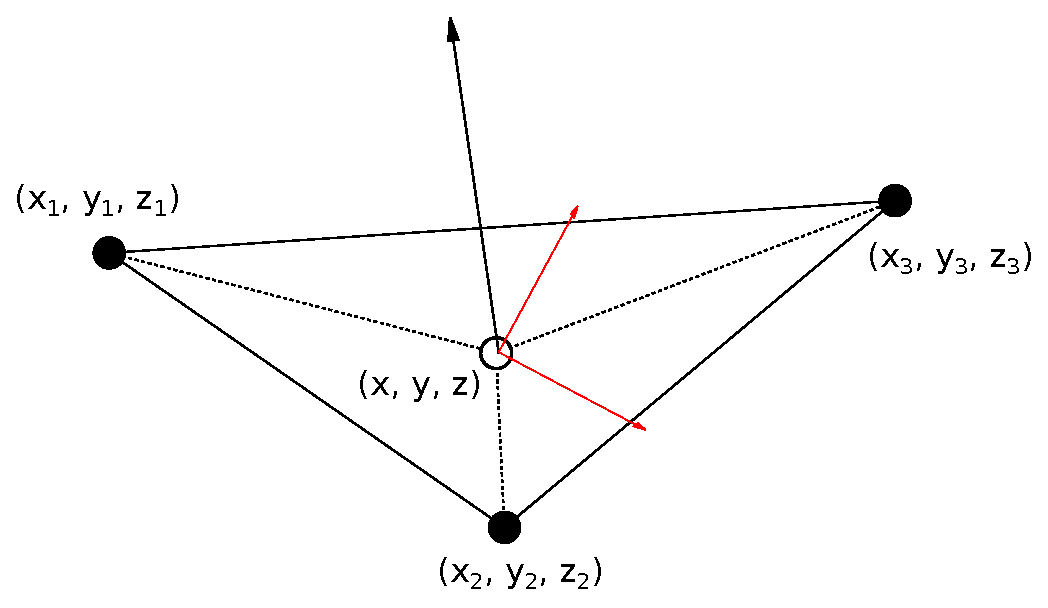
\includegraphics[width=0.6\textwidth]{eps/triangle_interpolation.eps}
\caption{Выбор новых осей координат при интерполяции в треугольнике}
\label{pic:triangle_interpolation}
\end{figure}
В работе используется следующий подход для реализации интерполяции:
\begin{itemize}
	\item поворотом осей координат добиваемся того, чтобы все четыре точки имели одинаковую координату $\tilde{x}$;
	\item используем интерполяцию в плоскости через барицентрические координаты.
\end{itemize}
Пусть $\vec{n}=(n_1,n_2,n_3)$ -- нормаль к плоскости треугольника, тогда в системе координат с базисными векторами:
\begin{eqnarray}
\label{eq:new_coords}
\vec{\tilde{e}}_1=(n_1, n_2, n_3), \nonumber \\
\vec{\tilde{e}}_2=(n_3, 0, -n_1), \nonumber \\
\vec{\tilde{e}}_3=(n_1*n_2, -n_1^2-n_3^2, n_2*n_3)
\end{eqnarray}
все четыре точки имеют одинаковую координату $\tilde{x}$. Такую систему координат невозможно использовать, если $n_1=n_3=0$, но в этом случае все точки имеют одинаковую координату $y$, поэтому сделав замену
\begin{eqnarray}
\label{eq:new_coords_2}
\tilde{x}=y \\
\tilde{y}=x \nonumber \\
\tilde{z}=z
\end{eqnarray}
придём опять к ситуации, когда все четыре точки имеют одинаковую координату $x$.
После этих преобразований значение в точке $(x,y,z)$ может быть вычислено по формуле
\begin{equation}
\label{eq:triangle_interpolation}
v=v_1*\lambda_1+v_2*\lambda_2+v_3*\lambda_3, 
\end{equation}
где $v_1,v_2,v_3$ -- значения в вершинах треугольника, а $\lambda_1,\lambda_2,\lambda_3$ -- барицентрические координаты
\begin{eqnarray}
\label{eq:barycentric_coords}
\lambda_1=\frac{(y_2-y_3)(x-x_3)+(x_3-x_2)(y-y_3)}{(y_2-y_3)(x_1-x_3)+(x_3-x_2)(y_1-y_3)}, \nonumber \\
\lambda_2=\frac{(y_3-y_1)(x-x_3)+(x_1-x_3)(y-y_3)}{(y_2-y_3)(x_1-x_3)+(x_3-x_2)(y_1-y_3)}, \nonumber \\
\lambda_3=1-\lambda_1-\lambda_2.
\end{eqnarray}
Эта интерполяция обладает первым порядком точности, что согласуется с порядком точности остальных частей алгоритма.
\subsubsection{Синхронизация тетраэдров}
Синхронизация тетраэдров необходима для реконструкции локальной топологии сетки, что требуется для правильного расчёта контактной границы. Идеи реализации схожи с теми, что были описаны выше:
\begin{itemize}
	\item вычислительный узел получает список треугольников, для которых нужно синхронизировать тетраэдры;
	\item по списку треугольников строится список тетраэдров, которые необходимо передать удалённому вычислительному узлу;
	\item создаётся пользовательский тип MPI и за одну пересылку осуществляется синхронизация тетраэдров.
\end{itemize}
\subsubsection{Производительность параллельной версии}
Для измерения производительности параллельной версии алгоритма были проведены расчёты одной и той же тестовой задачи на разном числе вычислительных узлов. В качестве тестовой задачи была взята задача о распространении волн в 24-слойной преграде. Каждый слой представляет собой прямоугольный параллелепипед размера 120x120x5 точек (86400 узлов, учитывая служебные, необходимые для восстановления локальной топологии удалённой сетки). На рисунках \ref{pic:gcm_boost} и \ref{pic:gcm_efficiency} представлены зависимости производительности и эффективности от числа используемых вычислительных узлов.
\begin{figure}[htp]
\centering
\includegraphics[width=0.6\textwidth]{eps/gcm3d-boost.eps}
\caption{Зависимость производительности от количества вычислительных узлов}
\label{pic:gcm_boost}
\end{figure}
\begin{figure}[htp]
\centering
\includegraphics[width=0.6\textwidth]{eps/gcm3d-efficiency.eps}
\caption{Зависимость эффективности использования кластера от количества вычислительных узлов}
\label{pic:gcm_efficiency}
\end{figure}
Таким образом при использовании параллельной версии алгоритма получено ускорение в 10 раз на 12 вычислительных узлах (эффективность использования кластера $\approx 83\%$). Этот результат является очень хорошим достижением.\todo{Почему?}
